\documentclass[10pt,a4paper]{report}
\usepackage[utf8]{inputenc}
\usepackage[T1]{fontenc}		% Allow underscore in text
\usepackage[english]{babel}
\usepackage{amsmath}
\usepackage{amsfonts}
\usepackage{amssymb}
\usepackage{graphicx}
\usepackage[backend=biber,firstinits=true,sorting=none]{biblatex}
\usepackage{csquotes}
\usepackage{siunitx}
\usepackage[font=small,labelfont=bf]{caption}
\usepackage{subcaption}
\usepackage{listings}
\usepackage{tikz}
\usepackage{tikzscale}
\usepackage{pgfplots}
\usepackage{color}
\usepackage{titlesec}
\usepackage{blindtext}
\usepackage{bm}
\usepackage{book tabs}
\usepackage{hyperref}

\graphicspath{ {figures/} }

\usetikzlibrary{positioning}
\tikzset{
	rect/.style={
	rectangle,
	minimum size=6mm,
	very thick,
	draw=white!20!black!80,
	top color=white,
	bottom color=white!50!black!20,
	% font=\itshape
	}
}

\pgfplotsset{compat=1.9}

\definecolor{codegreen}{rgb}{0,0.6,0}
\definecolor{codegray}{rgb}{0.5,0.5,0.5}
\definecolor{codepurple}{rgb}{0.58,0,0.82}
\definecolor{backcolour}{rgb}{0.95,0.95,0.92}
\definecolor{codeorange}{rgb}{0.95,0.45,0}
\lstdefinestyle{mystyle}{
    backgroundcolor=\color{backcolour},   
    commentstyle=\color{codegreen},
    keywordstyle=\color{magenta},
    numberstyle=\tiny\color{codegray},
    stringstyle=\color{codeorange},
    % basicstyle=\footnotesize,
    basicstyle=\ttfamily\small,
    breakatwhitespace=false,         
    breaklines=true,                 
    captionpos=b,                    
    keepspaces=true,                 
    numbers=left,                    
    numbersep=5pt,                  
    showspaces=false,                
    showstringspaces=false,
    showtabs=false,                  
    tabsize=2
}
\lstset{style=mystyle}

\definecolor{gray75}{gray}{0.75}
\newcommand{\hsp}{\hspace{20pt}}
\titleformat
	{\chapter}			% command
	[hang]				% shape
	{\Huge\bfseries}	% format
	{\thechapter\hsp\textcolor{gray75}{|}\hsp} % label
	{5pt}				% sep
	{\Huge\bfseries}	% before code


\author{André Hedlund}
\title{Effective Finite Element Analysis Workflow for Structural Mechanics}

\bibliography{thesis.bib}

\begin{document}
\maketitle
\begin{abstract}
%!TEX root = report.tex

The Finite Element Method (FEM) is a technique for finding the approximate solution of differential equations. It is commonly used in structural analysis to evaluate the deformation and internal stresses of a structure that is subject to outer loads. This thesis investigates the Finite Element Analysis (FEA) workflow that is used at Andritz Hydro AB, with the objective to find solutions that make the workflow more effective. The current workflow utilises \textit{Siemens NX} and \textit{Salomé} for pre- and post-processing, and \textit{Code Aster} as the FEM solver. Two different approaches that improve the workflow are presented. The first suggest that the entire FEA workflow is migrated to NX using the built-in FEM package of NX called \textit{Advanced Simulation}. The second approach utilises the Salomé API (Application Programming Interface) to create a customised toolbox (a script containing several functions) that automate several repetitive and cumbersome steps of the workflow, therefore effectively reducing the time that is required by the analyst to perform FEA. Due to the effective results and ease-of-use, the Salomé toolbox is preferred over the license cost and steep learning curve that is related to NX and Advanced Simulation. 

\end{abstract}
\tableofcontents

%!TEX root = report.tex

\chapter{Introduction}
\label{cha:introdution}

% \subsection{Hydro-Electric Power}
Hydro-power is the worlds largest renewable energy source, and hydroelectric power plants have been developed and used since the nineteenth century. During the last decade hydro-power amount to 45 percent of the total electricity production in Sweden~\cite{scb}. Many of the hydro-power plants in Sweden were built several decades ago, and they are therefore in need of refurbishment and modernisation. A simplified description of a conventional hydro power plant is that it consist of a dam, turbine and a generator, where the dam creates a water reservoir that contains potential energy that drives the turbine which in turn generates electricity.

% \subsection{Andritz Hydro}
The ANDRITZ GROUP provides services mainly for the hydro-power, pulp and paper, and metals industries, with headquarters in Graz, Austria and approximately \num{24500} employees worldwide. ANDRITZ HYDRO is a supplier of electromechanical equipment for hydro-power plants, and the Swedish subsidiary ANDRITZ HYDRO AB has 160 employees and focuses mainly on refurbishment and optimisation of turbines and generators.

% Write about the 'product realization process'
Turbines and generators are advanced electromechanical equipment, and since hydroelectric power plants need to reliably operate under long terms, the modernisation process is subject to rigorous analysis to ensure long term operation. At ANDRITZ HYDRO AB the entire realisation process with design, analysis and manufacturing is performed. 
%TODO: Expand this section by explaining in more detail PLM and structural analysis.
The design process is done with CAD (Computer Aided Design) and most of the analysis with CAE (Computer Aided Engineering). Siemens NX software is a design, engineering and manufacturing solution, and at Andritz Hydro AB it is mainly used for CAD. For the analysis the Salome platform is used with Code Aster as solver.

%TODO: Write more about machined parts and that the focus of this thesis I on the analysis of new parts.

% Write about why the workflow is problematic at Andritz
In general, a significant amount of time is spent on preparing model for the simulation -- usually more than the actual solver run -- it is therefore important to make the pre-processing as effective as possible.

At Andritz Hydro AB the workflow of the modernization process is in some aspects cumbersome and convoluted, and a more streamlined workflow is desired. Some of the difficulties occur solely because of that two different software programs are used for CAD and CAE, and other difficulties are generically inherited from the software programs that are used.

The main purpose of this thesis is to evaluate the current workflow at Andritz Hydro AB, and suggest changes to the workflow that will improve the analysis. The first evaluation of the workflow is concerned with larger strategical improvements, such as integrating the design and analysis process to the same software. The second evaluation is concerned with smaller improvements that try to simplify cumbersome processes within a specific software.

Since the product realisation process is complex, it is not certain that there exist feasible solutions that improves the workflow. It is also not guaranteed that the software programs provides functionality such that processes can be simplified.


%\subsection{Finite Element Analysis}
%
%\subsection{Finite Element Analysis at ANDRITZ} \label{sec:feaandritz}
%
%When a part is subject to an analysis the calculation engineer start with a part in NX. The part is idealised by removing smaller holes, chamfers and fillets that are non-essential for the analysis. Idealising the part can be done with the synchronous modelling commands that are available in NX. The part is now exported as a \texttt{.step} file that contains the geometrical description of the part.
%
%The \texttt{.step} file is imported into Salome-Meca a software platform for pre- and postprocessing. The idealisation that is done in NX is the first step in the preprocessing of the part. The next step is to create the necessary groups where boundary conditions and loads will be applied. The final step of the preprocess is to mesh the part, the part needs to be divided into a set of elements that describe the original model in accurately. The part is now exported from Salome-Meca, a text file that describes the geometry, the mesh and the defined groups is produced.
%
%The next part of the analyses is to solve the case by first defining the boundary conditions, load cases and physical properties that are needed to create a tractable model. These steps are done with command-line driven open source FEM package called Code Aster. The text file that Salome-Meca produced describes the geometry, mesh and groups that adheres to the \texttt{.unv} format, this format is not preferred by Code Aster, therefore the \texttt{.unv} file is converted to a \texttt{.mail} file. The case setup is described in a \texttt{.comm} file that is read by Code Aster.
%
%The post-processing is performed in Salome-Meca where the results created by Code Aster is imported. The final analysis of the results are visualised as needed.
%
%\begin{figure}
%	\centering
%	\rule{2cm}{2cm}
%	\label{fig:workflow}
%	\caption{A schematic figure of the workflow at ANDRITZ HYDRO AB for finite element analyses.}
%\end{figure}
%
%\subsection{Goal}
%The main focus of this thesis is to investigate the possibility to imporove this workflow process, to see if any changes are possible and if they would improve efficiency. There are several perspectives that could be investigated, and the main focus of this thesis will be on:
%\begin{itemize}
%	\item NX provides a utility called \emph{Advanced Simulation} that includes the functionality to both create groups and mesh from NX. If \emph{Advanced Simulation} fulfils the requirements of the current process, it would be possible to eliminate several steps from the workflow that is described in section~\ref{sec:feaandritz} and Figure~\ref{fig:workflow}.
%	\item \emph{Advanced Simulation} also includes the functionality to use some of the eminent solvers Nastran, Abaqus and Ansys. Therefore it is of interest to investigate how this functionality works in NX.
%\end{itemize}
%Eventhough the focus of the investigation is to evaluate the technical functionalities of NX and \emph{Advanced Simulation}, it is important to establish that the current NX license that is used at ANDRITZ HYDRO AB does not include the \emph{Advanced Simulation} utility. Therefore, the investigated paths described above would result in an increase of the costs, since the current softwares (Salome-Meca and Code Aster) are open source and free of charge.
%
%The investigation will also take another perspective, which is to try and improve the current workflow, without changing any of the main steps. The current workflow contains several exports and imports between different softwares and a general analysis could include several iterations between the calculation team and the design team. During these iterations, small, but significant changes are made on the part that is under analysis. Due to the convoluted workflow it is difficult to reuse the settings and work done on the previous part, therefore the process has to be repeated even if just a small change has been done to the part. This is particularly evident in the preprocessing step in Salome-Meca, where the defined groups and mesh settings are lost between these iterations. 
%
%Salome-Meca provides a python API (Application Programming Interface) such that the user might create its own scripts to perform tasks that are not provided by Salome-Meca. With this functionality it is possible to investigate if a script can be written such that it can compare the part from the previous iteration with the new part to see if some of the groups and meshes can be copied to the new part. If this is possible then it would eliminate the nuisance of having to recreate the settings between the iterations.
%
%
%






%!TEX root = report.tex

\section{Theory} % (fold)
\label{sec:theory}
This section gives a basic introduction to the Finite Element Method (FEM) for structural mechanics, and describes the different stages of finite element analysis (FEA). It also describes the current analysis workflow at Andritz Hydro AB, highlighting the processes that are necessary to streamline. After the workflow description follows a presentation of the software that are utilized for analysis at Andritz Hydro AB.

\subsection{Finite Element Method for Structural Mechanics} % (fold)
\label{sub:finite_element_method_in_structural_mechanics}
Here follows a short but descriptive text about FEM.
When, where and why did it originate?
Elements
Mathematical formulation
System of equations

During the design of structures it is important to analyse if the structure is capable of supporting the applied loads; structural mechanics focuses on the computation of deformations and stresses, to evaluate the performance of the structure. The physical phenomena that are investigated (stress, strain, elasticity etc.) are modelled by differential equations together with a set of boundary conditions. Generally, there exist no analytical solutions to differential equations that relate to complex structures, therefore, the only way to solve the equations are with numerical methods.

The finite element method is as numerical approach that can be used to approximate the solution of boundary value problems. The method has been used rigorously in different engineering disciplines for several decades, and its main advantage over other numerical methods for solving differential equations is its capability to handle complex geometries. The structure is divided into smaller parts, called elements, which together create a discrete mesh of the geometry.~\cite{ottossen92}

(Maybe add section with mathematical FEM description. degrees of freedom)


\subsubsection{Pre-Processing} % (fold)
\label{ssub:pre_processing}
When a structure has been designed the CAD model needs to be analysed to determine if the desired performance qualifications are reached. The first step of the analysis is the pre-processing, which prepares the model for a computation.

% Clean: FEA book p. 181-191
Ideally, the CAD model built by the design team is usable for finite element analysis without having to alter the model, this is however often not the case. It is often necessary to make simplifications to the model in order to create a mesh of the model. Design features that complicate automatic meshing are short edges, sliver faces, small holes, fillets, chamfers etc., and it is necessary to clean the model of these features to enable the automesher to mesh the model. This cleaning process can be both tedious and difficult since it may exist a lot of features and even if a disadvantageous feature is found it may be difficult to remove it; the cleaning process can therefore be very time consuming. It is also important to mention that the simplifications that is performed should not influence the structural capabilities of the model, this could be difficult to assess, but as long as the simplifications are local and not in areas of interest.~\cite[p.~181--191]{adams99}

% Meshing
When the model is clean, the next step is to mesh the model. Whether the model is meshed automatically or manually and with shell elements or tetrahedrons, the process is an essential step of the analysis. The focus of this thesis is on automeshing with tetrahedrons (for 3D models) and triangles (for 2D models). Automeshing is a simple technique to create a discrete FE model of the CAD model. Depending on which automesher that is used different settings are available, but the user should generally consider the maximum and minimum elements size, growth rate and local mesh refinements. The goal is to create a mesh that captures the structural features of the model with as few elements as possible. Even though the automesher could create the mesh in a fast and convenient way, it is no guarantee that the mesh is sufficiently refined. Therefore, considerable thought should be spent on where local mesh refinements are necessary, how small elements are needed and how large elements are excepted. It is also important to mention that it is an absolute necessity that the model is clean, otherwise the automesher will most likely fail to create a mesh.~\cite[p.~251-255]{adams99}

Part of the pre-process is also to define the boundary conditions that influence the model. There exist two groups of boundary conditions: constraints that prohibits the model of rigid body motion, that is remove spatial degrees of freedom, and loads such as forces, moments and temperature. How the boundary condition are defined and which types that are used are often not straightforward, and an important part of the analysis.~\cite[p.~263]{adams99}

Before the FE model can be solved the material properties of the model needs to be specified.

It is probably obvious that this part of the analysis can be very time consuming, and to obtain a solution it is of paramount importance that the FE model is created correctly, with sufficient details of the original model and that boundary conditions are properly defined.
% subsubsection pre_processing (end)

\subsubsection{Solution} % (fold)
\label{ssub:solution}
When the FE model is created, the next step is to solve the model to obtain the results. This step is mainly executed by the computer, the only effort from the user is setting the correct solver parameters. Which parameters that can be specified is highly dependent on which solver is used. The execution time depends on how large the FE model is (number degrees of freedom) and what solution type is used (non-linear solutions are more demanding).

When the solver is finished it is important to evaluate the results and the solver output to establish if the solution is reasonable and if the results are accurate. To determine if the mesh is sufficiently refined the convergence could be checked, and to check that the boundary conditions are properly defined the resultant forces on the model could be compared with the specified loads.~\cite[p.~303-324]{adams99}
% subsubsection solution (end)

\subsubsection{Post-Processing} % (fold)
\label{ssub:post_processing}
The post-processing first visualise the results (displacement, stress, etc.) to determine if the results are reasonable, then the specific results that are looked for are determined. Even if this step is not very technical, it is important to analyse the results to determine if the reuslts can be trusted.
% subsubsection post_processing (end)

\subsubsection{Elements} % (fold)
\label{ssub:elements}
Describe different types of elements.
% subsubsection elements (end)

\subsubsection{Boundary Condidtions} % (fold)
\label{ssub:boundary_condidtions}
Describe different types of bc's.
% subsubsection boundary_condidtions (end)

\subsubsection{Load Cases} % (fold)
\label{ssub:load_cases}
Maybe not necessary
% subsubsection load_cases (end)

\subsubsection{Contacts} % (fold)
\label{ssub:contacts}
Describe non-linearity, meshing technique etc.
% subsubsection contacts (end)

% subsection finite_element_method_in_structural_mechanics (end)

\subsection{Siemens NX} % (fold)
\label{sub:siemens_nx}
Write some general about NX and which features that are used. Also write about Advanced Simulation.
% subsection siemens_nx (end)

\subsection{Salomé Platform} % (fold)
\label{sub:salom_platform}
Write about the platform and the possibilities it offers.
% subsection salom_platform (end)

% section theory (end)

%!TEX root = report.tex

\chapter{Analysis} % (fold)
\label{cha:analysis}
The previous section described structural analysis and FEA in general and presented different software programs that can be used in the analysis. This section presents how FEA is performed at Andritz Hydro AB based on the investigation made by the author of this thesis. The investigation is the basis of the improvement suggestions that are given in sourcethis section.

\section{Analysis Workflow at Andritz} % (fold)
\label{sec:analysis_workflow_at_andritz}
% Product development process: FEA p. 12-13
The structural analysis begins with a CAD model created by the design team. The design engineers at Andritz Hydro AB use Siemens NX to create CAD models, internally in NX these models are called \textit{parts}. The parts are given a reference number to a database where they are stored, and this reference number is passed on to the calculation team. As described in Section~\ref{sub:pre_processing}, the CAD model needs to be cleaned of features that are unnecessary to the analysis. Since the cleaning process can change the model significantly it is not appreciated by the design engineers that the model they created is altered, therefore, a copy of this model is created which can be prepared for analysis. A copy is created by creating a new part in the database that is assigned to the calculation engineer and then using a synchronous modelling tool called \textit{WAVE Geometry Linker} to link the part created by the design engineer.

The cleaning process is done in NX with the synchronous modelling tools that is described in Section~\ref{sec:siemens_nx}. Depending on the level of detail of the model that is provided, the amount of work that is needed on the cleaning process can range from very little to a significant part of the entire analysis process. 

When the part is ready to be meshed it is exported from NX. There exists several formats to export a CAD model such that the details of the model are preserved, and at Andritz the STEP (standard for the exchange of product model data) format is used. A STEP file describes a CAD model according to an ISO standard which is used for file exchange~\cite{stepiso}.

The rest of the pre-processing is carried out in the Salomé Platform described in Section~\ref{sec:salom_platform}. The STEP file is imported and the Geometry module is selected. As described in Section~\ref{sub:geometry_module}, groups are created in the Geometry module to define where local mesh refinement is needed, where boundary conditions are applied and possible contact surfaces.

After the groups are defined the the analyst change to the Mesh module where the model is meshed. The meshing process in Salomé is described in Section~\ref{sub:mesh_module}. 3D models are usually meshed with tetrahedrons (see Sec.~\ref{sub:elements}) and 2D models are usually meshed with triangles, in both cases the NETGEN algorithm is used.

To solve the model Code Aster is used and, as is described in Section~\ref{sec:code_aster}, Code Aster requires the mesh to be described in a text file where patches, on which boundary conditions are applied, are defined. Therefore, mesh groups are defined in the Mesh module before the mesh is exported.

The final steps of the analysis (solution and post-processing) has not been investigated to the same level of detail, and are therefore summarised just to give a complete description of the analysis workflow. Given a file describing the mesh and a COMM file that describes the simulation, Code\_Aster can run the simulation. The COMM file describes the type of simulation, boundary conditions and other parameters depending on the type of simulation. The output of the simulation is the results that can be visualised and analysed with the ParaVis module.

The workflow described is presented in Figure~\ref{fig:andritz_workflow}. 

\begin{figure}[t]
	\begin{center}
		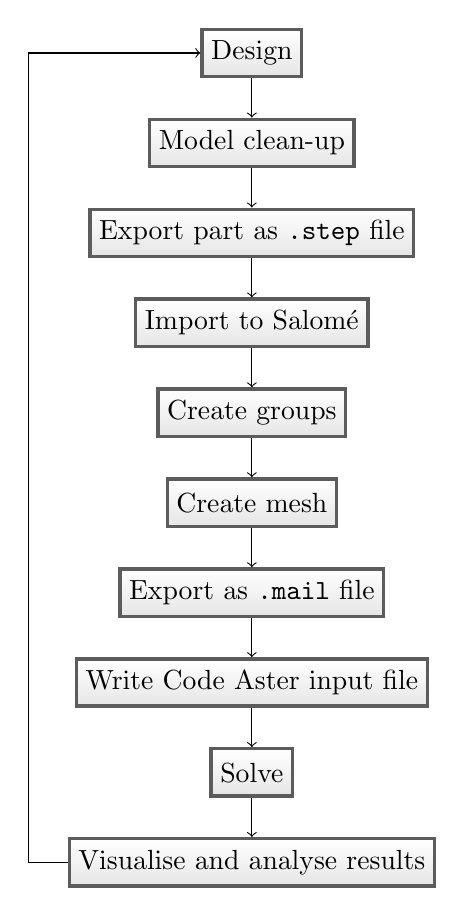
\begin{tikzpicture}[node distance=5mm]
			\node[rect] (design)					{Design};
			\node[rect] (clean)	[below=of design] 	{Model clean-up};
			\node[rect] (step)	[below=of clean]	{Export part as \texttt{.step} file};
			\node[rect] (salom)	[below=of step]		{Import to Salomé};
			\node[rect] (group) [below=of salom] 	{Create groups};
			\node[rect] (mesh)	[below=of group]	{Create mesh};
			\node[rect] (mail)	[below=of mesh]		{Export as \texttt{.mail} file};
			\node[rect] (comm)	[below=of mail]		{Write Code Aster input file};
			\node[rect] (solve)	[below=of comm]		{Solve};
			\node[rect] (vis)	[below=of solve]	{Visualise and analyse results};
			\path (design)	edge[->]	(clean)
				  (clean)	edge[->]	(step)
				  (step)	edge[->]	(salom)
				  (salom)	edge[->]	(group)
				  (group)	edge[->]	(mesh)
				  (mesh)	edge[->]	(mail)
				  (mail)	edge[->]	(comm)
				  (comm)	edge[->]	(solve)
				  (solve)	edge[->]	(vis);
			\draw [->] (vis.west) -- ++(-.5,0) |- (design.west);
		\end{tikzpicture}
	\end{center}
	\caption{Current analysis workflow at Andritz Hydro AB.}
	\label{fig:andritz_workflow}
\end{figure}

If the results are feasible the development of the CAD model can continue, and preparations for the manufacturing process can begin. However, if the results show that the model does not fulfil the requirements the model needs to be redesigned and the analysis repeated on the updated model. This iteration procedure is standard in product development. Since the analysis of the updated model is likely to be very similar to the original model some of the steps described in Figure~\ref{fig:andritz_workflow} are reusable, however, some steps have to be performed again. During the analysis of a redesigned model the following steps cannot be reused:
\begin{itemize}
	\item Model clean-up
	\item Create geometric groups
	\item Create mesh
	\item Create mesh groups
\end{itemize}
Obviously the visualisation and analysis of the results need to be repeated, but that is unavoidable. The four steps mentioned above are all part of the pre-process of the analysis, and they could be a very time consuming part of the analysis, so it would be favourable to find a solution that could reuse the fact that these steps already have been performed on a very similar model. 

It is also possible that half way through the analysis there could be an update to the original CAD model that is independent of the analysis. If the update is significant to the analysis a new analysis needs to be started in this case as well. This is because the link between the CAD model and the analysis model is broken during the first step when the CAD model is copied. This is obviously very frustrating and time consuming for the analyst. Since these updates of the CAD model are impossible to prevent a solution that diminish the effect of the update is very desirable.
% subsection analysis_workflow_at_andritz (end)

\section{Using NX Advanced Simulation} % (fold)
\label{sec:using_nx_advanced_simulation}
The previous section described the structural analysis workflow at Andritz Hydro AB and highlighting parts of the workflow that is inefficient, especially if a new iteration is started. This section describes a possible solution to some of the problems that are discussed. NX Advanced Simulation (described in Sec.~\ref{sec:siemens_nx}) supports the entire FEA process 

Suggested workflow with NX Advanced Simulation:

\begin{figure}[t]
	\begin{center}
		\includegraphics{WAVEGeometryLinker}
	\end{center}
	\caption{WAVE Geometry Linker dialogue box in NX.}
	\label{fig:WAVEGeometryLinker}
\end{figure}
% subsection using_nx_advanced_simulation (end)

\section{Salomé API Script} % (fold)
\label{sec:salom_api_script}
Salomé provides a Python API for every module that allows the user to write Python scripts to automate processes that are often repeated. As is described in Section~\ref{sec:analysis_workflow_at_andritz}, there are steps in the pre-process of the FEA workflow that can be time consuming to perform manually, and it is especially inefficient if a new iteration is started since the steps that already have been done, must be repeated. This section presents a solution that efficiently automate some parts of the pre-processing steps and at the same time reduces the amount of work that have to be repeated if a new iteration is started.

The main issue with the workflow in Figure~\ref{fig:andritz_workflow} is that the connection between the CAD model and the FE model is lost when the part is exported from NX and imported to Salomé. All the steps of the pre-processing that is done in Salomé needs to be repeated with the current workflow. Therefore, it would be better to move as many of the steps as possible from Salomé to NX, since these steps would not have to be repeated. Within the current NX license at Andritz Hydro AB, the step that can be moved is the definition of the groups.

The main idea of the new workflow is to clean the model and define the groups in NX, and when the model is exported the group definitions are included in the STEP file. In Salomé the model is imported and the groups defined in NX are automatically created. The model is meshed and the groups that should be included in the text file describing the mesh are automatically created in the Mesh module.

\subsubsection{Defining Groups in NX} % (fold)
\label{ssub:defining_groups_in_nx}
In NX any geometrical object (solid, face, edge, etc.) or collection of objects can be given a name. The name and which geometrical object it is associated with are included in the STEP file when the model is exported. The import utility in Salomé does not recognise these names as groups when the STEP file is imported, therefore these names needs to be manually translated to group objects. The Geometry API provides several functions to automate this process, and the solution is a function named \texttt{CreateGroups} which is presented in Appendix~\ref{sec:creategroups}. \texttt{CreateGroups} creates the groups that are defined in NX of the object that is selected in the object browser.

The \textit{Explode} function creates sub-shapes of a specified type of an object, for example if a box is exploded to faces all eight faces of the box are created. Using this function the groups defined in NX can be recreated.

See example in Figure~\ref{fig:example1}.

\begin{figure}[t]
	
\begin{subfigure}{.3\textwidth}
	\begin{center}
		\includegraphics{Untitled}
	\end{center}
	\caption{Object browser}
	\label{fig:objbrow}
\end{subfigure}
\begin{subfigure}{.7\textwidth}
	\begin{center}
		\includegraphics[trim=10 80 50 0,clip,scale=.5]{example.png}
	\end{center}
	\caption{A simple example.}
	\label{fig:example1}
\end{subfigure}

	\caption{Caption here}
	\label{fig:figure1}
\end{figure}


% subsubsection defining_groups_in_nx (end)

% The proposed workflow is presented in Figure~\ref{fig:script_workflow}.

% \begin{figure}[t]
% 	\begin{center}
% 		\begin{tikzpicture}[node distance=5mm]
% 			\node[rect] (design)					{Design};
% 			\node[rect] (clean)	[below=of design] 	{Model clean-up};
% 			\node[rect] (group) [below=of salom] 	{Create groups};
% 			\node[rect] (step)	[below=of clean]	{Export part as \texttt{.step} file};
% 			\node[rect] (salom)	[below=of step]		{Import to Salomé};
% 			\node[rect] (mesh)	[below=of group]	{Create mesh};
% 			\node[rect] (mail)	[below=of mesh]		{Export as \texttt{.mail} file};
% 			\node[rect] (comm)	[below=of mail]		{Write Code Aster input file};
% 			\node[rect] (solve)	[below=of comm]		{Solve};
% 			\node[rect] (vis)	[below=of solve]	{Visualise and analyse results};
% 			\path (design)	edge[->]	(clean)
% 				  (clean)	edge[->]	(step)
% 				  (step)	edge[->]	(salom)
% 				  (salom)	edge[->]	(group)
% 				  (group)	edge[->]	(mesh)
% 				  (mesh)	edge[->]	(mail)
% 				  (mail)	edge[->]	(comm)
% 				  (comm)	edge[->]	(solve)
% 				  (solve)	edge[->]	(vis);
% 			\draw [->] (vis.west) -- ++(-.5,0) |- (design.west);
% 		\end{tikzpicture}
% 	\end{center}
% 	\caption{Current analysis workflow at Andritz Hydro AB.}
% 	\label{fig:script_workflow}
% \end{figure}
% subsection salom_api_script (end)




% section analysis (end)

%!TEX root = report.tex

\chapter{Conclusions} % (fold)
\label{sec:conclusions}

\section{NX Advanced Simulation} % (fold)
\label{sub:nx_advanced_simulation}
Present Advanced Simulation.
% subsection nx_advanced_simulation (end)

% \subsection{Salomé API Script} % (fold)
% \label{sub:salom_api_script}
% Present the script.
% % subsection salom_api_script (end)



% section conclusions (end)

%!TEX root = report.tex

\chapter{Acknowledgements} % (fold)
\label{cha:acknowledgement}

I would like to thank my supervisor at Andritz Hydro AB Mikael Helin for providing me with the subject of this thesis, and for his guidance and experience to help me develop the final product. I would also like to thank Tobias Marten at Andritz Hydro AB for taking his time to answer my questions and guiding me in the right direction. Finally, I would like to thank Per Isaksson at Uppsala University for taking his time to read my thesis and quickly providing me with feedback.

% chapter acknowledgement (end)


\printbibliography

%!TEX root = report.tex

\chapter{Appendix} % (fold)
\label{cha:appendix}

\section{NX Advanced Simulation Guide} % (fold)
\label{sec:nx_advanced_simulation_guide}
TODO: Put guide here.

% \begin{figure}[t]
% 	\begin{center}
% 		\includegraphics{WAVEGeometryLinker}
% 	\end{center}
% 	\caption{WAVE Geometry Linker dialogue box in NX.}
% 	\label{fig:WAVEGeometryLinker}
% \end{figure}
% section nx_advanced_simulation_guide (end)

\section{\texttt{CreateGroups}} % (fold)
\label{sec:creategroups}
\lstinputlisting[language=Python]{codesnippets/creategroups.py}
\subsection{\texttt{GetNXGroups}} % (fold)
\label{sub:getnxgroups}
\lstinputlisting[language=Python]{codesnippets/getnxgroups.py}
% subsection getnxgroups (end)
% section creategroups (end)

\section{\texttt{CreateMesh}} % (fold)
\label{sec:createmesh}
\lstinputlisting[language=Python]{codesnippets/createmesh.py}
\subsection{\texttt{CreateAlgorithm}} % (fold)
\label{sub:createalgorithm}
\lstinputlisting[language=Python]{codesnippets/createalgorithm.py}
% subsection createalgorithm (end)
% section createmesh (end)

\section{\texttt{PartitionShapes}} % (fold)
\label{sec:partitionshapes}
\lstinputlisting[language=Python]{codesnippets/partitionshapes.py}
\subsection{CreateTreeStructure} % (fold)
\label{sub:createtreestructure}
\lstinputlisting[language=Python]{codesnippets/createtreestructure.py}
% subsection createtreestructure (end)
\subsection{MoveContactGroups} % (fold)
\label{sub:movecontactgroups}
\lstinputlisting[language=Python]{codesnippets/movecontactgroups.py}
% subsection movecontactgroups (end)
\subsection{MoveOtherGroups} % (fold)
\label{sub:moveothergroups}
\lstinputlisting[language=Python]{codesnippets/moveothergroups.py}
% subsection moveothergroups (end)
% section partitionshapes (end)

\section{\texttt{CreateSubMesh}} % (fold)
\label{sec:createsubmesh}
\lstinputlisting[language=Python]{codesnippets/createsubmesh.py}
% section createsubmesh (end)

% chapter appendix (end)



\end{document}

